\documentclass[11pt]{article}

\usepackage{times}
\usepackage{epsf}
\usepackage{epsfig}
\usepackage{amsmath, alltt, amssymb, xspace}
\usepackage{wrapfig}
\usepackage{fancyhdr}
\usepackage{url}
\usepackage{verbatim}
\usepackage{fancyvrb}

\usepackage{subfigure}
\usepackage{cite}
%\usepackage{cases}
%\usepackage{ltexpprt}
%\usepackage{verbatim}

%\topmargin      -0.70in  % distance to headers
%\headheight     0.2in   % height of header box
%\headsep        0.4in   % distance to top line
%\footskip       0.3in   % distance from bottom line

% Horizontal alignment
\topmargin      -0.50in  % distance to headers
\oddsidemargin  0.0in
\evensidemargin 0.0in
\textwidth      6.5in
\textheight     8.9in 


%\centerfigcaptionstrue

%\def\baselinestretch{0.95}


\newcommand\discuss[1]{\{\textbf{Discuss:} \textit{#1}\}}
%\newcommand\todo[1]{\vspace{0.1in}\{\textbf{Todo:} \textit{#1}\}\vspace{0.1in}}
\newtheorem{problem}{Problem}[section]
%\newtheorem{theorem}{Theorem}
%\newtheorem{fact}{Fact}
\newtheorem{define}{Definition}[section]
%\newtheorem{analysis}{Analysis}
\newcommand\vspacenoindent{\vspace{0.1in} \noindent}

%\newenvironment{proof}{\noindent {\bf Proof}.}{\hspace*{\fill}~\mbox{\rule[0pt]{1.3ex}{1.3ex}}}
%\newcommand\todo[1]{\vspace{0.1in}\{\textbf{Todo:} \textit{#1}\}\vspace{0.1in}}

%\newcommand\reducespace{\vspace{-0.1in}}
% reduce the space between lines
%\def\baselinestretch{0.95}

\newcommand{\fixmefn}[1]{ \footnote{\sf\ \ \fbox{FIXME} #1} }
\newcommand{\todo}[1]{
\vspace{0.1in}
\fbox{\parbox{6in}{TODO: #1}}
\vspace{0.1in}
}

\newcommand{\mybox}[1]{
\vspace{0.2in}
\noindent
\fbox{\parbox{6.5in}{#1}}
\vspace{0.1in}
}


\newcounter{question}
\setcounter{question}{1}

\newcommand{\myquestion} {{\vspace{0.1in} \noindent \bf Question \arabic{question}:} \addtocounter{question}{1} \,}

\newcommand{\myproblem} {{\noindent \bf Problem \arabic{question}:} \addtocounter{question}{1} \,}


\newcommand{\copyrightnoticeA}[1]{
\vspace{0.1in}
\fbox{\parbox{6in}{\small Copyright \copyright\ 2006 - 2014\ \ Wenliang Du, Syracuse University.\\ 
      The development of this document is partially funded by 
      the National Science Foundation's Course, Curriculum, and Laboratory 
      Improvement (CCLI) program under Award No. 0618680 and 0231122. 
      Permission is granted to copy, distribute and/or modify this document
      under the terms of the GNU Free Documentation License, Version 1.2
      or any later version published by the Free Software Foundation.
      A copy of the license can be found at http://www.gnu.org/licenses/fdl.html.}}
\vspace{0.1in}
}


\newcommand{\copyrightnotice}[1]{
\vspace{0.1in}
\fbox{\parbox{6in}{\small Copyright \copyright\ 2006 - 2014\ \ Wenliang Du, Syracuse University.\\
      The development of this document is/was funded by three grants from
      the US National Science Foundation: Awards No. 0231122 and 0618680 from
      TUES/CCLI and  Award No. 1017771 from Trustworthy Computing.
      This lab was imported into the Labtainer framework by the Naval Postgraduate 
      School, Center for Cybersecurity and Cyber Operations under National Science 
      Foundation Award No. 1438893.
      Permission is granted to copy, distribute and/or modify this document
      under the terms of the GNU Free Documentation License, Version 1.2
      or any later version published by the Free Software Foundation.
      A copy of the license can be found at http://www.gnu.org/licenses/fdl.html.}}
\vspace{0.1in}
}

\newcommand{\copyrightnoticeB}[1]{
\vspace{0.1in}
\fbox{\parbox{6in}{\small Copyright \copyright\ 2006 - 2014\ \ Wenliang Du, Syracuse University.\\
      The development of this document is/was funded by the following grants from
      the US National Science Foundation: No. 0231122, 0618680, and 1303306.
      Permission is granted to copy, distribute and/or modify this document
      under the terms of the GNU Free Documentation License, Version 1.2
      or any later version published by the Free Software Foundation.
      A copy of the license can be found at http://www.gnu.org/licenses/fdl.html.}}
\vspace{0.1in}
}


\newcommand{\nocopyrightnotice}[1]{
\vspace{0.1in}
\fbox{\parbox{6in}{\small  
      The development of this document is funded by 
      the National Science Foundation's Course, Curriculum, and Laboratory 
      Improvement (CCLI) program under Award No. 0618680 and 0231122. 
      Permission is granted to copy, distribute and/or modify this document.
      }}
\vspace{0.1in}
}

\newcommand{\idea}[1]{
\vspace{0.1in}
{\sf IDEA:\ \ \fbox{\parbox{5in}{#1}}}
\vspace{0.1in}
}

\newcommand{\questionblock}[1]{
\vspace{0.1in}
\fbox{\parbox{6in}{#1}}
\vspace{0.1in}
}


\newcommand{\minix}{{\tt Minix}\xspace}
\newcommand{\unix}{{\tt Unix}\xspace}
\newcommand{\linux}{{\tt Linux}\xspace}
\newcommand{\ubuntu}{{\tt Ubuntu}\xspace}
\newcommand{\selinux}{{\tt SELinux}\xspace}
\newcommand{\freebsd}{{\tt FreeBSD}\xspace}
\newcommand{\solaris}{{\tt Solaris}\xspace}
\newcommand{\windowsnt}{{\tt Windows NT}\xspace}
\newcommand{\setuid}{{\tt Set-UID}\xspace}
%\newcommand{\smx}{{\tt Smx}\xspace}
\newcommand{\smx}{{\tt Minix}\xspace}
\newcommand{\relay}{{\tt relay}\xspace}
\newcommand{\isys}{{\tt iSYS}\xspace}
\newcommand{\ilan}{{\tt iLAN}\xspace}
\newcommand{\iSYS}{{\tt iSYS}\xspace}
\newcommand{\iLAN}{{\tt iLAN}\xspace}
\newcommand{\iLANs}{{\tt iLAN}s\xspace}
\newcommand{\bochs}{{\tt Bochs}\xspace}

\newcommand\FF{{\mathcal{F}}}

\newcommand{\argmax}[1]{
\begin{minipage}[t]{1.25cm}\parskip-1ex\begin{center}
argmax
#1
\end{center}\end{minipage}
\;
}

\newcommand{\bm}{\boldmath}
\newcommand  {\bx}    {\mbox{\boldmath $x$}}
\newcommand  {\by}    {\mbox{\boldmath $y$}}
\newcommand  {\br}    {\mbox{\boldmath $r$}}


%\pagestyle{fancyplain}
%\lhead[\thepage]{\thesection}      % Note the different brackets!
%\rhead[\thesection]{SEED Laboratories}
%\lfoot[\fancyplain{}{}]{Syracuse University} 
%\cfoot[\fancyplain{}{}]{\thepage} 

\newcommand{\tstamp}{\today}   
%\lhead[\fancyplain{}{\thepage}]         {\fancyplain{}{\rightmark}}
%\chead[\fancyplain{}{}]                 {\fancyplain{}{}}
%\rhead[\fancyplain{}{\rightmark}]       {\fancyplain{}{\thepage}}
%\lfoot[\fancyplain{}{}]                 {\fancyplain{\tstamp}{\tstamp}}
%\cfoot[\fancyplain{\thepage}{}]         {\fancyplain{\thepage}{}}
%\rfoot[\fancyplain{\tstamp} {\tstamp}]  {\fancyplain{}{}}

\pagestyle{fancy}
%\lhead{\bfseries Computer Security Course Project}
\lhead{\bfseries SEED Labs}
\chead{}
\rhead{\small \thepage}
\lfoot{}
\cfoot{}
\rfoot{}

\usepackage{listings}
\usepackage{color}

\definecolor{dkgreen}{rgb}{0,0.6,0}
\definecolor{gray}{rgb}{0.5,0.5,0.5}
\definecolor{mauve}{rgb}{0.58,0,0.82}

\lstset{frame=tb,
  language=C,
  aboveskip=3mm,
  belowskip=3mm,
  showstringspaces=false,
  columns=flexible,
  basicstyle={\small\ttfamily},
  numbers=none,
  numberstyle=\tiny\color{gray},
  keywordstyle=\color{blue},
  commentstyle=\color{dkgreen},
  stringstyle=\color{mauve},
  breaklines=true,
  breakatwhitespace=true,
  tabsize=3
}



\begin{document}

\begin{center}
{\LARGE SSH-Agent}
\vspace{0.1in}\\
\end{center}


\section{Overview}
This lab illustrates the use of an SSH agent to manage private keys used to
authenticate to SSH services on Linux computers.  The goal is to allow a user
to use SSH to securely authenticate from the client to a local server, and then from the
local server to a remote server, without providing either a password or a passphrase,
(after initial setup and initialization of an SSH Agent).

\subsection {Background}
A previous lab, \textit{sshlab},
illustrated the use of public and private keys for SSH authentication.  This lab
will show how to protect those private keys with a passphrase, but without having
to type in the passphrase each time you wish to access a remote system.

The student is expected to have some familiarity with the Linux command line,
the basics of the file system, and the ability to locate and edit a file.  

\section{Lab Environment}
This lab runs in the Labtainer framework,
available at http://my.nps.edu/web/c3o/labtainers.
That site includes links to a pre-built virtual machine
that has Labtainers installed, however Labtainers can
be run on any Linux host that supports Docker containers.

From your labtainer-student directory start the lab using:
\begin{verbatim}
    labtainer ssh-agent
\end{verbatim}
\noindent A link to this lab manual will be displayed.  


\section{Network Configuration}
This lab includes a client computer, a local server and
a remote server as shown in Figure~\ref{fig:topology}.
When the lab starts, you will get one virtual terminal connected 
to the client.


\begin{figure}[H]
\begin{center}
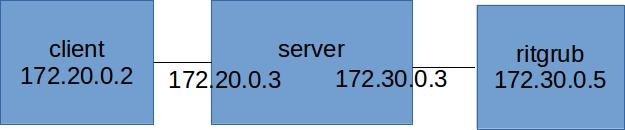
\includegraphics [width=0.8\textwidth]{ssh-agent.jpg}
\end{center}
\caption{Network topology for the SSH-Agent lab}
\label{fig:topology}
\end{figure}

\section{Lab Tasks}
\subsection{Explore}
Use ssh to authenticate to the local server, and then from there to the
remote server named {\tt ritgrub}.  The user ID and password are ``ubuntu''.
Then use exit, twice, to return to the client's shell.

\subsection{Generate and copy keys}
Use the ssh-keygen command to generate a public and private key pair on the client computer.
\begin{verbatim}
ssh-keygen -t rsa
\end{verbatim}
\noindent When prompted for a passphrase, provide one and make note if it.  Recall
that in the {\tt sshlab}, you left the passphrase blank, which is convenient but
not very secure.

Copy the public key to the server's {\tt authorized\_keys} file.  This directs the
server's SSH service to accept proof of possession of the corresponding private key as a
basis for authenticating the user:
\begin{verbatim}
ssh-copy-id -i ~/.ssh/id_rsa.pub server
\end{verbatim}

You should now be able to SSH from the client to the server without providing the password,
though you will be prompted for the passphrase that you provided to protect the private key.
\begin{verbatim}
ssh server
\end{verbatim}
\noindent While still in a session on the server, you will now copy your {\tt authorized\_keys}
file to the {\tt ritgrub} server.
\begin{verbatim}
scp -r ~/.ssh ritgrub:~/
\end{verbatim}
\noindent This directs the {\tt ritgrub} server's
SSH service to accept proof of possession of the corresponding private key as a
basis for authenticating the user.  Note however that the private key will never exist
on the local server.

\subsection{Start an SSH Agent to manage your private key}
Use {\tt exit} to return to the client.
Then use these commands to start an SSH agent on the client, and provide that agent with access to your
new private key:
\begin{verbatim}
eval `ssh-agent`	
ssh-add
\end{verbatim}
\noindent Note the argument to the {\tt eval} command is enclosed in back-tics (upper left on
most keyboards.)  When prompted, provide the passphrase used to protect your private key.
Then SSH to the local server again.  You should be able to do so without providing a passphrase.
\begin{verbatim}
ssh server
\end{verbatim}

Accessing the {\tt ritgrub} server from the local server still requires a password, because the
local server is unable to prove that the requesting user possesses the private key.  We can rectify
this by exiting from the local server back to the client, and restarting the SSH session, but with the 
{\tt -A} option:
\begin{verbatim}
ssh -A server
\end{verbatim}
\noindent
This option enables forwarding of the SSH agent connection.  When you SSH to a remote host that
recognizes the public key in its 
\begin{verbatim}
~/.ssh/authorized\_keys
\end{verbatim}
\noindent file, the SSH agent on the client will
be used to prove possession of the private key.  You should now be able to SSH from the local server to
the gitrub server without a password.  Try it, and then exit back to the client.

\subsection{Use an SSH config file to enable agent forwarding}
The SSH program references a file named 
\begin{verbatim}
~/.ssh/config
\end{verbatim}
\noindent (if it exists), to get defaults and
configuration settings for each SSH session.  This file can be configured so that you need not remember
to add the {\tt -A} option to the ssh command. Each entry in this file begins with a {\tt Host} line
that identifies the hostname you will use in the SSH command, and that is typically followed by a
{\tt HostName} line that includes the DNS name or IP address of that host.  The entry then includes
configuration information, in our case, an indication that we want to enable agent forwarding.  Such
an entry might look like:
\begin{verbatim}
Host server
   HostName server
   ForwardAgent yes
\end{verbatim}
\noindent
Create a {\tt config} file and demonstrate your ability to SSH from the client to the server, and
then on to the ritgrub server without passphrases, passwords, or use of an explicit {\tt -A} option.

\section{Submission}
After finishing the lab, go to the terminal on your Linux system that was used to start the lab and type:
\begin{verbatim}
    stoplab 
\end{verbatim}
When you stop the lab, the system will display a path to the zipped lab results on your Linux system.  Provide that file to 
your instructor, e.g., via the Sakai site.

\end{document}
